\setcounter{section}{6}

\Needspace{5\baselineskip}
\hypertarget{dueling-dqn}{%
\section{Dueling DQN}\label{dueling-dqn}}

In DQN, \(Q\) depends jointly on state \(s\) and action \(a\). In some states, however, the agent needs only to know ``whether the current environment is good'' (the \(V\) value), regardless of differences between actions. Only when actions must avoid danger or earn points does it need to know ``which action is better than average'' (the \(A\) value). Modeling these separately lets \(V(s)\) focus on the overall situation, assessing whether the environment is good, while \(A(s,a)\) focuses on details, assessing which actions are better and by how much. This decoupling allows \(V(s)\) to be learned and updated from every sample (because \(V(s)\) is the foundation whichever action is chosen), substantially improving training efficiency.

\begin{figure}[htbp]
\centering
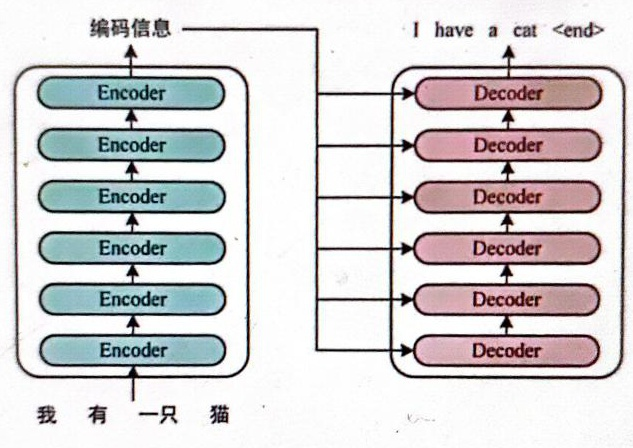
\includegraphics{images/image-0015.jpeg}
\caption{Intuitive distinction between state value and action advantage in Dueling DQN}
\end{figure}

Scenario A (a long straight road without cars ahead): the screen (state \(s\)) suggests a stable situation likely to yield a high score. Steering slightly left or right (action \(a\)) has little effect on the final score.

\begin{itemize}
\tightlist
\item
  Conclusion: \(V(s)\) (state value) is high, while differences in \(A(s,a)\) (action advantage) are small. The network need not laboriously learn each action's specific value; knowing ``this is a good place'' is enough.
\end{itemize}

Scenario B (an obstacle ahead requiring a sharp turn): state \(s\) is dangerous, and poor control causes a crash.

\begin{itemize}
\tightlist
\item
  Conclusion: action selection is crucial. Turning left may lead to survival and right to failure, so differences in action advantage \(A(s,a)\) are large.
\Needspace{5\baselineskip}
  We therefore split Q as:
\end{itemize}

\[
Q(s,a;\theta,\alpha,\beta)=V(s;\theta,\beta)+A(s,a;\theta,\alpha)
\]

\begin{itemize}
\tightlist
\item
  \(\theta\): shared parameters (convolutional layers), extracting general image features such as edges, shapes, and object positions, useful both for assessing the situation and choosing actions.
\item
  \(\beta\): value-stream parameters (fully connected layers), mapping features to scalar \(V\).
\item
  \(\alpha\): advantage-stream parameters (fully connected layers), mapping features to vector \(A\) with dimension equal to the number of actions.
  The problem is that we calculate and update \(Q\) values: how can \(V\) and \(A\) be recovered from \(Q\)?
\end{itemize}

Enumerate all actions \(a'\) in the same state \(s\). Their relative \(Q\) values also give their relative \(A\) values. One solution, for a given \(s\), takes action \(a^*\) maximizing \(Q(s,a')\), sets \(A(s,a^*)=0\) (the maximum advantage), and \(V(s)=Q(s,a^*)\):

Option A: max constraint (theoretically optimal)

\[
Q(s,a)=V(s)+(A(s,a)-\max_{a'}A(s,a'))
\]

\begin{itemize}
\tightlist
\item
  Mathematical meaning: force the maximum advantage to \(0\).
\Needspace{5\baselineskip}
  Another solution sets the mean advantage over all actions to 0:
\end{itemize}

Option B: mean constraint (optimal in engineering practice)

\[
Q(s,a)=V(s)+(A(s,a)-\frac{1}{|\mathcal{A}|}\sum_{a'}A(s,a'))
\]

\begin{itemize}
\item
  Mathematical meaning: force the sum of all advantages to \(0\), equivalently their mean to \(0\).
\item
  Why it is better: \(\max\) is nonlinear, passing gradients only at the maximum and giving gradients of \(0\) elsewhere; the mean sums all actions, allowing smooth gradient flow to every action-advantage output node.
\item
  Noise resistance: the mean is less sensitive to outliers, stabilizing training.
\Needspace{5\baselineskip}
  Although this does not strictly satisfy the Bellman optimality equation, it is better in engineering practice, for the following reasons:
\item
  Mathematical meaning: force the sum of all advantages to \(0\) (equivalently their mean to \(0\)).
\item
\Needspace{5\baselineskip}
  Why it is better:

  \begin{itemize}
  \tightlist
  \item
    Gradient stability: \(\max\) is nonlinear, passing gradients only at the maximum and giving gradients of \(0\) elsewhere. The mean sums all actions, allowing smooth gradient flow to every action-advantage output node.
  \item
    Noise resistance: the mean is less sensitive to outliers, stabilizing training.
  \end{itemize}
\end{itemize}

\FloatBarrier
\Needspace{5\baselineskip}
\hypertarget{references-52}{%
\subsection{References}\label{references-52}}

\vspace{0.25em}
\begin{itemize}
\tightlist
\item
  Wang, Z., Schaul, T., Hessel, M., van Hasselt, H., Lanctot, M., \& de Freitas, N. (2016). \href{https://arxiv.org/abs/1511.06581}{Dueling Network Architectures for Deep Reinforcement Learning}. ICML 2016.
\item
  \href{https://hrl.boyuai.com/}{Hands-on Reinforcement Learning (translated title; in Chinese)}.
\end{itemize}

\clearpage
